%*******************************************************************************
%*********************************** First Chapter *****************************
%*******************************************************************************

\chapter{Introduction}  %Title of the First Chapter
\label{cha:intro}

% **************************** Define Graphics Path **************************
\ifpdf
    \graphicspath{{Chapter1/Pics/Raster/}{Chapter1/Pics/PDF/}{Chapter1/}}
\else
    \graphicspath{{Chapter1/Pics/Vector/}{Chapter1/}}
\fi



%-< SECTION >--------------------------------------------------------------------
\section{Motivations}
\label{sec:intro_motivations}
%\begin{itemize}[noitemsep,topsep=0pt]
%    \item Nowadays Internet has scalability issue and lacks of flexibility.
%    \item Due to Internet problems, LISP is proposed.
%    \item State LISP current status.
%    \item As LISP is still in infancy, which kinds of works are need to do to move LISP forward.
%\end{itemize}

%-< FIGURE >--------------------------------------------------------------------
\begin{figure}[t]
	\centering
	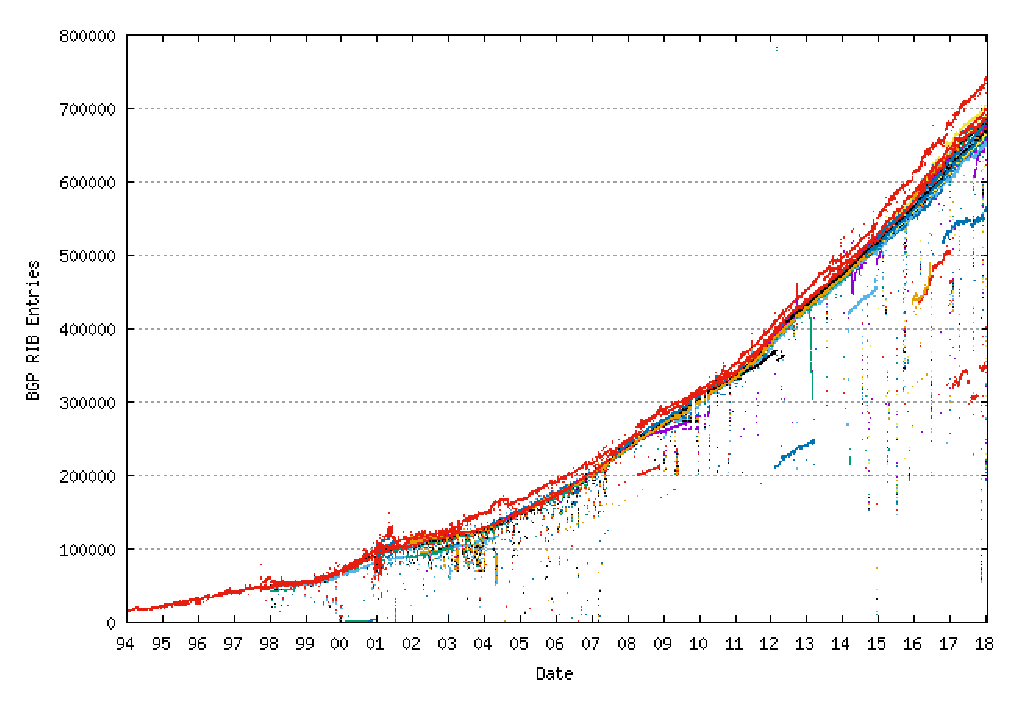
\includegraphics[width=0.8\textwidth]{Pics/Growth_BGP_Table.eps}
	\caption{Growth of the BGP Table - 1994 to Present~\cite{bgptableanalysis}}
	\label{Growth_BGP_Table}
\end{figure}
%-< END FIGURE >--------------------------------------------------------------------
Since the \acrshort{arpanet} (\acrlong{arpanet}) emerged in 1966~\cite{marill1966toward}, the Internet has obtained significant achievements over the last fifty years and developed very fast. At the beginning of 2018, the Internet users in the world are 3.82 billions, i.e., around 40\% of the world population has an Internet connection today~\cite{InternetLiveStats}. Moreover, we come into the era of the mobile Internet. According to the latest research~\cite{SmartInsights}, the number of global mobile users has been higher than that of desktop since 2014. Although having a huge success, today's Internet is suffering the overloading of IP address semantic, which results in many shortcomings in the application landscape~\cite{feng2017locator}. In the current TCP/IP protocol stack, the IP address serves both as the \emph{who} to identify the host and the \emph{where} to indicate the attachment point in the network topology, leading to a serious routing scalability problem. As shown in Fig.~\ref{Growth_BGP_Table}, the BGP table size, which is the number of IP prefixes in the \acrshort{bgp} (\acrlong{bgp}) routing table of \acrshort{dfz} (\acrlong{dfz}) routers, has grown at a super-linear rate in recent years. After full use of IPv6, the routing scalability issue will be aggravated, since it has much larger addressing space than IPv4. Maintaining such routing table is very cumbersome, since once a site changes its routing information, all the routers need to update, which causes a huge BGP churn. In addition, frequent routing information updates result in the increase of convergence time and packet loss rates.

To cope with the current Internet scalability problems, the Loc/ID separation paradigm is proposed, which separates the single IP addressing space into two orthogonal spaces. Many solutions based on this mechanism are proposed, which can be classified into two categories: \emph{Host-based} and \emph{Network-based}. The former one needs to modify the host stack. The representative architectures are: HIP (Host Identity Protocol)~\cite{nikander2010host}~\cite{Moskowitz2017host}~\cite{moskowitz2015host}, Six/One~\cite{vogt2007six}, SHIM6 (Site Multihoming by IPv6 Intermediation)~\cite{garcia2010shim6}~\cite{nordmark2009shim6}, ILNP (Identifier-Locator Network Protocol)~\cite{bhatti2012identifier}~\cite{atkinson2010evolving}, and LNA (Layered Naming Architecture)~\cite{balakrishnan2004layered}. The network-based approach needs to update the routers, and the representative proposals are: GSE (Global, Site, and End-system address elements)~\cite{o2006gse}, LISP (Locator/ID Separation Protocol)~\cite{rfc6830}, and TIDR (Tunneled Inter-domain Routing)~\cite{adan2006tunneled}. Among them, LISP is outstanding by its relatively comprehensive network systems in both control and data planes. % This characterization promotes the standardization, production and industrtialization of LISP. 
LISP was initially proposed by Cisco in 2006 and has an exclusive IETF WG since 2009. % which guarantees LISP can be actively under developed.

The key philosophy of LISP is to separate the IP addressing space into two sub-spaces: the \emph{Routing LOCators} (RLOCs) and the \emph{Endpoint IDentifiers} (EIDs). End-to-end communication is based on EIDs, which in an intra-domain context means just performing conventional routing and forwarding. On the contrary, for inter-domain end-to-end communication, RLOCs are used for routing and forwarding. To this end, LISP does a map-and-encap operation, first mapping EIDs to RLOCs (through a DNS-like on-demand \acrfull{mds}\footnote{The terms \emph{\acrfull{mds}} and the \emph{mapping system} are used interchangeably in this dissertation.}~\cite{lispALTPourri}) and then encapsulating the original packet so to use RLOCs on the outer header. Internetworking between LISP and non-LISP networks is performed through two types of proxies~\cite{rfc6832}: \emph{Proxy Ingress Tunnel Routers} (PITRs) and \emph{Proxy Egress Tunnel Routers} (PETRs). They are collectively denoted by \emph{PxTR}. PITRs advertise in the BGP  routing infrastructure the EID-prefix space on behalf of the LISP sites, so that non-LISP sites can reach them. % In this way PITRs attract the traffic from non-LISP sites, which simply send packets with destination EID as destination IP address. Subsequently the PITR performs LISP encapsulation and forward the packets to the destination. 
PETRs are used as exit points from LISP sites when the destination is not an EID in a LISP site. % Hence, PETRs decapsulate the LISP-encapsualted packets received from LISP-sites and forwards them in the legacy Internet. 
With help of this mechanism, LISP is able to improve the Internet routing scalability, enable enhanced inter-domain traffic engineering, lightweight multi-tenant carrier-grade VPN, and \acrshort{vm}s mobility in Data-Centers~\cite{saucez2012designing}.

% LISP introduces several benefits to the Internet architecture. Many companies and academic institutes participate into LISP development, so that the standardizations and research publications about LISP are continuously came out in the recent years. Besides, two large scale experimental LISP platforms are deployed on the world respectively in 2008 and 2015. All the efforts, however, are mainly about the description of LISP architectures, implementations, extensions and applications. It lacks of the comprehensive LISP measurement works from the various aspects. In addition, LISP remains a relatively recent technology and these large scale flexible platforms are still in an early stage, it needs plenty of large scale experiments to obtain realistic LISP experiences ont only further improve the performance of two platforms, but ultimately to provide feedback to the community on how to move the LISP technology forward.

As LISP is a promising technology that brings many benefits to the Internet, it attracts the attention from both academic and industrial world. Many companies, universities and research institutes are now involved in the development of LISP. Hence, the related standardization and research are very active. In terms of deployment, two large-scale experimental LISP platforms: LISP Beta Network and LISP-Lab platform are deployed on the world respectively in 2008 and 2015. Up to date, all the efforts are mainly about theoretic or simulation-based performance analysis, description of LISP architectures, implementations, extensions, applications and so on. However, it lacks of the comprehensive measurement works for LISP technology itself. These performance measurements work will give the research community a clear view about the LISP performance, reveal the points that can be improved, indicate possible research directions, and improve the performance of two platforms. Thus, the large-scale measurements in realistic networks are of paramount importance for the LISP development.

%-< SECTION >--------------------------------------------------------------------
\section{Contributions}
\label{sec:intro_contributions}
With the goal of evaluating LISP from the different views, in this dissertation we aim at answering the following research questions, which have not been tackled before:
\begin{enumerate}[noitemsep,topsep=0pt]
	\item Mapping system is essential in LISP, because it decides where the packets will be routed. Thus, does it always provide the identical mapping information for the same destination? Do all of the \acrlong{mr}s (\acrshort{mr}s) of the mapping system offer the same response at the same time? Does the mapping information replies keep consistent if we query them from the different \acrlong{vp}s (\acrshort{vp}s)?
	
	We continuously measured LISP Beta Network for seventeen days. Measurements show that the LISP mapping system is stable over most of time. The replies from the different \acrshort{mr}s and \acrshort{vp}s are also mostly consistent. Nevertheless, instability and inconsistency are observed although they are rare events. We define a new taxonomy to classify these instabilities and inconsistencies so to facilitate a deeper analysis. This work is published in WNM~\cite{yue2016stability}.
	
	\item As the results of the last question show that there exists inconsistency between the \acrshort{mr}s and \acrshort{vp}s, is it possible to implement a comprehensive monitor so to simultaneously supervise the whole mapping system and all the resolvers?
	
	We propose a dynamic LISP monitoring architecture, namely LISP-Views, so to deepen the understandings on LISP and to ease day-to-day operations and troubleshooting. After one full month monitoring the whole LISP mapping system, it demonstrates that LISP-Views provides % more information by discovering more mapping information from all \acrshort{mr}s and more 
	the complete mapping information. Furthermore, with our proposed monitoring platform, more mapping system performance metrics such as reliability, latency, and configuration issues can be assessed, which helps for further LISP improvements. This work is published in ITC~\cite{li2017lisp}.
	
	\item By using proxy approach to communicate with the legacy Internet, a stretch in the path is introduced. How much is it in the real world performance when the platforms integrate with the legacy Internet? Under which conditions such stretch has an important impact on the performance? Conversely, under which situation such overhead is so small that it can be ignored? 
	
	To evaluate LISP interworking performance with legacy Internet, we conduct two measurement campaigns. The results of the two experiments are coherent. Both of them show that LISP is stable although the stretch is introduced due to the use of proxies. We find that the proxy indeed introduces negative effects for the destinations located in Europe and America, but can be ignored for the intercontinental long-distance transmissions to Asia destinations. Besides, we observe that the position of proxies is very important. If it is either near to the sources or the destinations can decrease the latency a lot. % Further, the performance of LISP-Lab PxTR is more reliable than the one of LISP Beta Network. 
	This work is published in INFOCOM Student workshop~\cite{li2016using}, ACM SIGCOMM Student workshop~\cite{li2016performance}, and Elsevier Computer Networks~\cite{Li2017}.
	
	\item As LISP separates the identifier and the topological attachment point from the traditional IP address, it is able to maintain the communication between two hosts during the handover. LISP can be implemented on the border routers or the terminals or even both of them. Thus, which network element supports LISP showing a better performance, i.e., having a shorter handover delay or introducing less overhead during the mobility? What are the advantages and shortcomings of each case? % Leveraging on which simulator can we verify?
	
	To explore the mobility performance of the LISP implementation on each network element, we design three different scenarios:
	\begin{inparaenum}[1)]
		\item Only mobile node supports LISP;
		\item Only border routers support LISP;
		\item Both mobile node and border routers support LISP.
	\end{inparaenum}
	The numerical analysis shows that the 1\textsuperscript{st} and 3\textsuperscript{rd} scenarios can achieve the mobile node roam through the different subnets, whereas they require additional permanent EID for each mobile node. The 1\textsuperscript{st} has no help on reducing the BGP table size and the 3\textsuperscript{rd} scenario shows much longer handover delay than the other two's. The 2\textsuperscript{nd} scenario presents the smallest handover delay and needs the least IP addresses, but it can only handle mobility within the same subnet. To verify the numerical analysis, we implement a LISP simulator with LISP mobility extensions under ns-3.27 by extending an existing ns-3 based LISP implementation.
	
\end{enumerate}	


%-< SECTION >--------------------------------------------------------------------
\section{Manuscript organization}
\label{sec:intro_structure}
%-< FIGURE >--------------------------------------------------------------------
\begin{figure}[t]
	\centering
	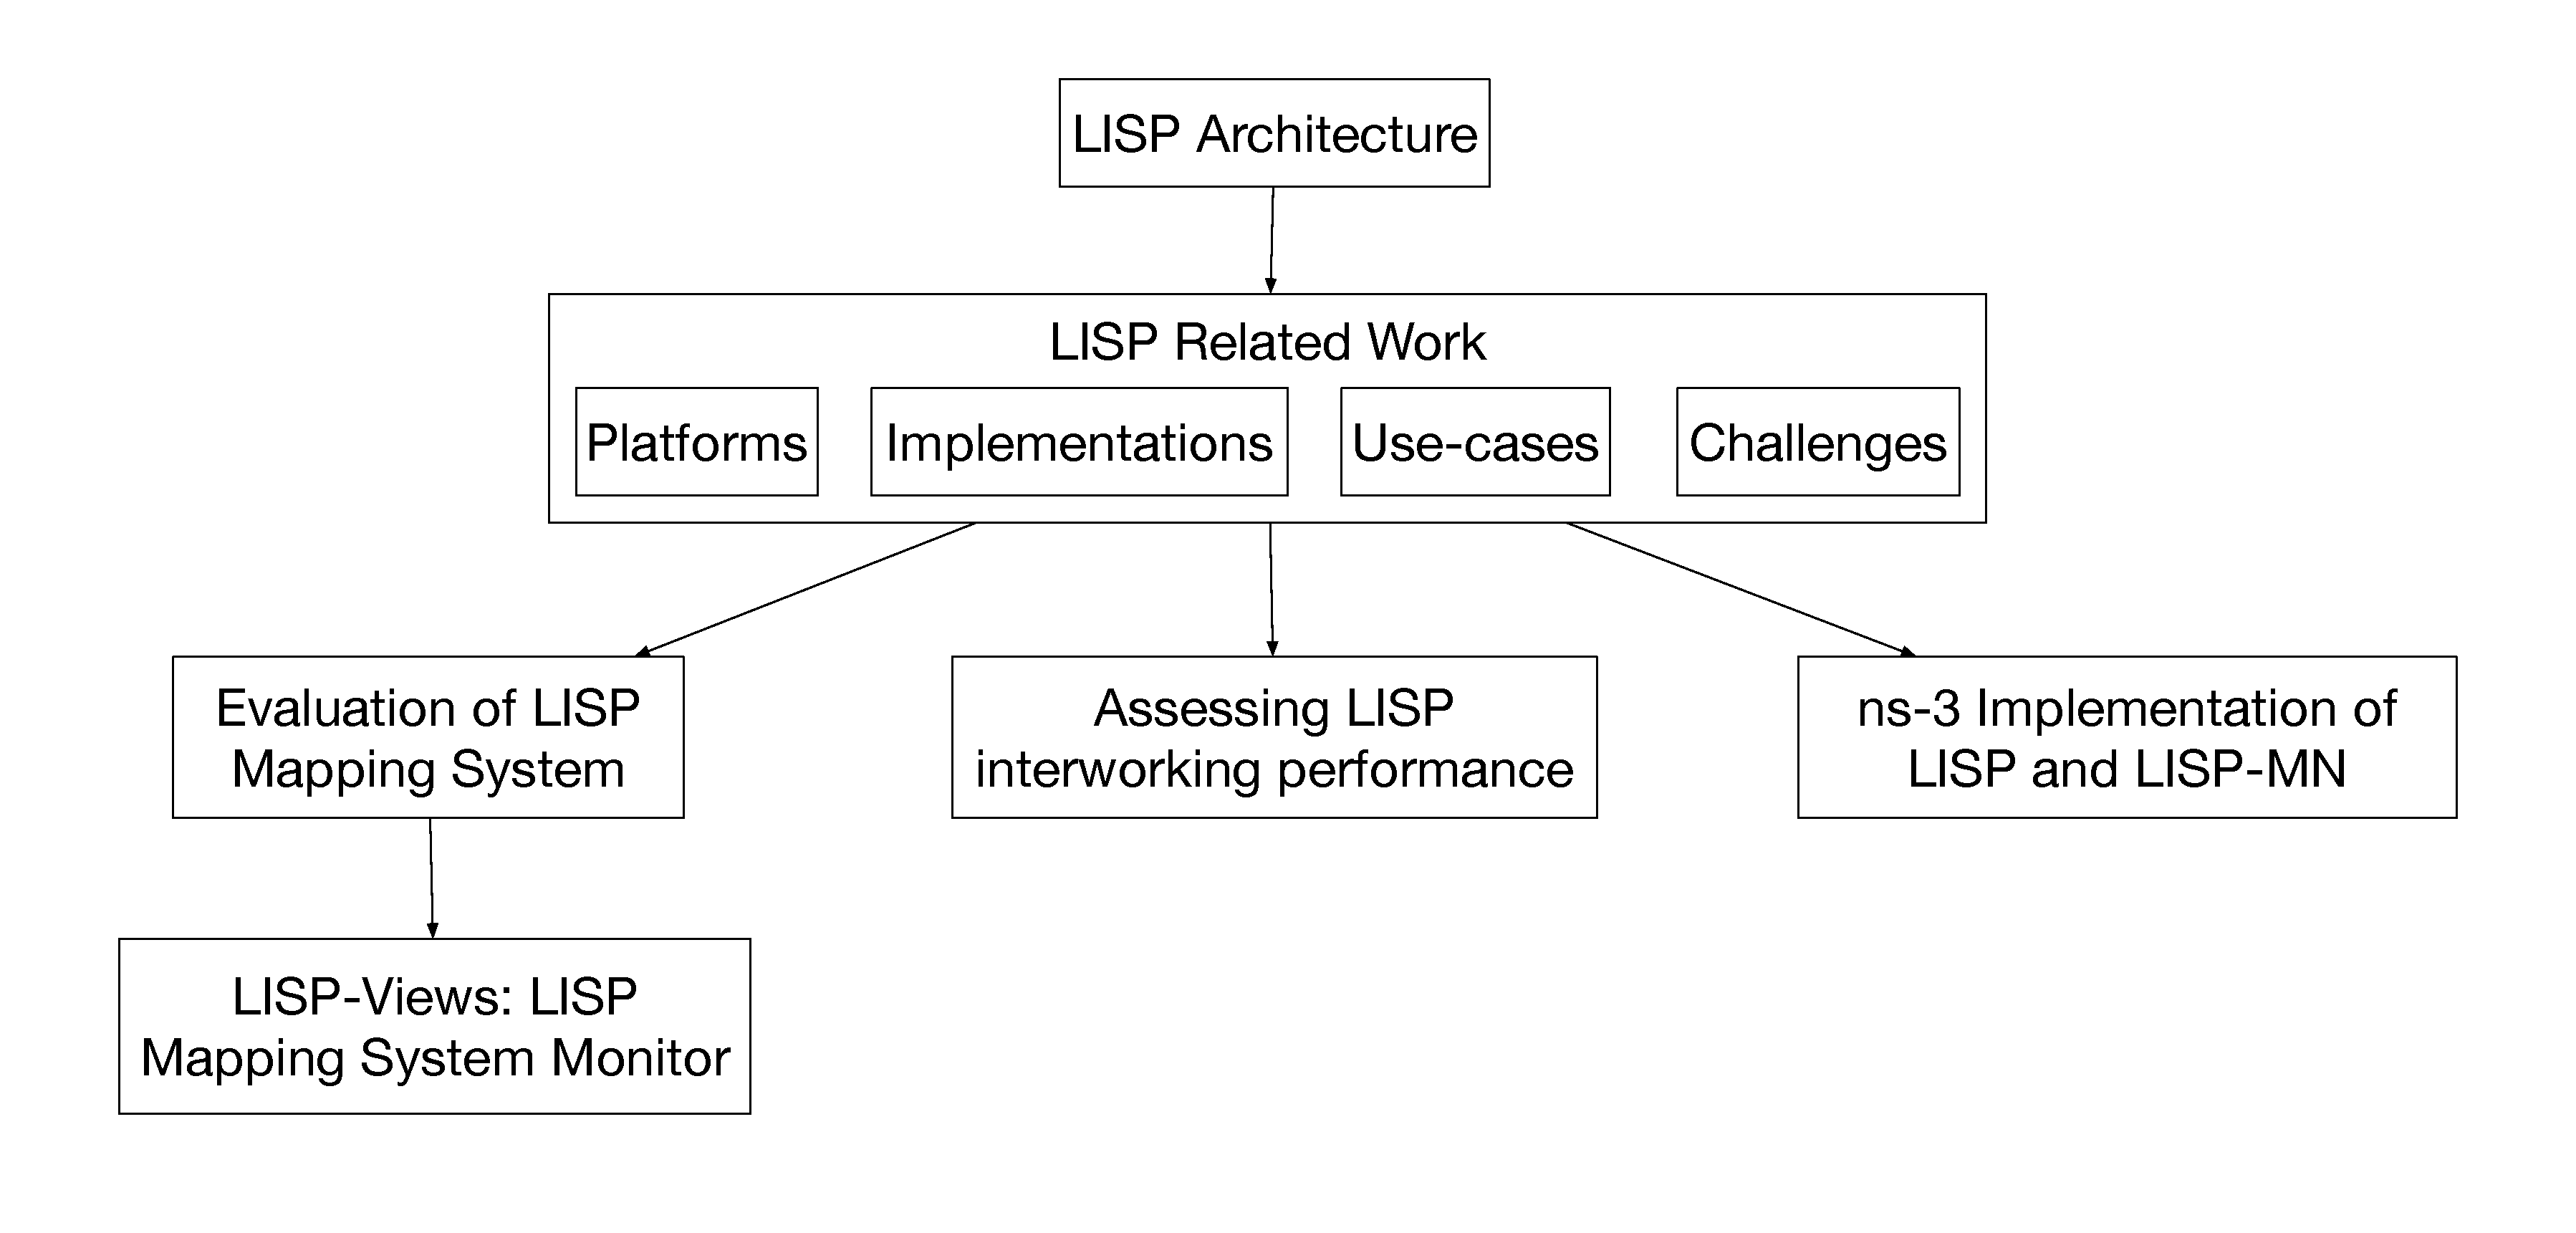
\includegraphics[width=\textwidth]{Pics/structure_thesis.eps}
	\caption{Structure of this dissertation}
	\label{structure_thesis}
\end{figure}
%-< END FIGURE >--------------------------------------------------------------------
The remainder of this dissertation is organized as follows and shown in Fig.~\ref{structure_thesis}:
\begin{itemize}[noitemsep,topsep=0pt]
	\item \emph{Chapter~\ref{cha:lisp_overview}}: Describes the basic LISP mechanisms, presenting how the packets are exchanged between two LISP-sites and with the legacy Internet. It also shows the different scenario of LISP mobility.
	\item \emph{Chapter~\ref{cha:related_work}}: The challenges brought by LISP, LISP-related studies and missing works are also illustrated. Introduces the LISP current status, such as: the available LISP platforms, the first LISP monitor, the LISP manual management tool, the open source LISP implementations and LISP use-cases.
    \item \emph{Chapter~\ref{cha:mds_evaluation}}: This chapter is about the evaluation of LISP Mapping System. In this chapter, we observe that if the mapping system always provides the same mapping information over time, and if we can obtain the identical mapping answers from the different network entities.
    \item \emph{Chapter~\ref{cha:LISPViews}}: Describes the proposition of LISP-Views: a LISP Mapping System Monitor at large scale. In this chapter, we introduce how this architecture is implemented, how it has been validated and what experimental results it can provide.
    \item \emph{Chapter~\ref{cha:pxtr}}: Assesses LISP interworking performance through RIPE Atlas. This chapter presents how the experiments are conducted, how much is the stretch introduced by proxy in the real world, and whether this stretch have a big impact on the performance or it can be ignored.
    \item \emph{Chapter~\ref{cha:ns-3}}: Introduces ns-3 Implementation of LISP mobility extension and numerically analyses the performance of different LISP mobility scenarios. In this chapter, we first describe how to implement the LISP mobility extension on the ns-3. Then we define three different LISP mobility scenarios, provide the numerical analysis of each scenario, and compare the advantages and shortcomings between them. 
    \item \emph{Chapter~\ref{cha:conclusion}}: Concludes the dissertation and discusses perspectives for further work.
\end{itemize}